%!TEX root = ../main.tex

\documentclass[../main.tex]{subfiles}
\begin{document}


\chapter{Single Agent Coverage}
\label{chapter:single_agent_coverage}

In this chapter, the problem of single agent coverage is formulated and a solution is proposed. The chapter is organized into six sections. Section~\ref{section:single_problem_statement} goes through a formulation of the problem. Section~\ref{section:min_alt_decomposition} proposes an algorithm. 
Section~\ref{section:single_agent_complexity} performs a computational complexity analysis. Section~\ref{section:single_agent_gtsp_tour} describes the formulation of the problem as a Generalized Traveling Salesman Problem. Lastly, Section~\ref{section:single_agent_simulation} presents the results of the algorithm in the form of simulations.

\section{Problem Statement}
\label{section:single_problem_statement}

The general coverage problem is defined in Problem~\ref{problem:min_cost_cpp}.
\begin{problem}[Minimum Cost Coverage Path Planning]
\label{problem:min_cost_cpp}
	Given a workspace $W$, a robot with dynamics, and a coverage footprint map $\mathcal{M}(q)$, compute a path $p_i$ such that
	\begin{equation}
	\label{condition:full_coverage}
	\begin{aligned}
		& p_i\in P,\\
		& \bigcup_{q\in p_i}\mathcal{M}(q)=\mathbb{C},\\
		& \mathcal{E}(p_i)\leq\mathcal{E}(p_j), \forall p_j\in P.
	\end{aligned}
	\end{equation}
\end{problem}

In Problem~\ref{problem:min_cost_cpp}, a workspace $W$, a robot with dynamics, and a coverage footprint map are given. The objective is to compute a path that lies entirely in the free configuration space of the robot such that the footprint of the whole path is equal to the coverable space and the cost of the path is minimized. A number of aspects of this problem makes it difficult. For instance, the set of feasible paths $W$ contains infinitely many paths. Also, it is difficult to directly check the satisfiability of conditions~(\ref{condition:full_coverage}). As such, several assumptions and heuristics are used throughout this work.

\begin{assumption}[Polygonal Workspace]
	The workspace is assumed to be polygonal,simply connected, and noise free. 
\end{assumption}

\begin{assumption}[General Robot Model Assumption]
	We deal with kinematic robot models with $v_{\max}$ as the maximum velocity. In Section~\ref{section:single_agent_simulation}, we utilize Dubins' car model for our simulations. We assume robot's coverage footprint is a circle of radius $r$. The localization problem is assumed to be solved. 
\end{assumption}


\subsection{Utilizing Segmented Paths}
\label{subsection:conversion_to_segmented}

\begin{assumption}[Reduced Set of Feasible Paths]
It is assumed that paths considered for coverage in this problem have a certain structure. The set of such paths is called a set of feasible segmented paths.
\end{assumption}

The set of feasible segmented paths is defined in Definition~\ref{definition:segmented_feasible_paths} with an example shown in Figure~\ref{fig:segmented}. Notably, these types of paths consists of a sequence of pairs of straight and transition segments.
\begin{definition}[Set of Feasible Segmented Paths]
\label{definition:segmented_feasible_paths}
A set of feasible segmented paths is defined as
	\begin{equation}
		P_{\text{segmented}}=\{p_i\ |\ p_i\subseteq Q_{\text{free}},\  p_i=\{s_1,t_1,s_2,t_2,\dots,s_n,t_n\}\},
	\end{equation}
	where $s_i$ refers to $i^{\text{th}}$ straight line segment and $t_i$ refers to $i^{\text{th}}$ transition segment.
\end{definition}

Problem~\ref{problem:min_cost_cpp} is modified accordingly with a modified search space of feasible paths.
\begin{problem}[Minimum Cost Coverage Path Planning with Straight Line Segments]
\label{problem:min_cost_cpp_with_lines}
	Given a workspace $W$, a robot with dynamics, and a coverage footprint map $\mathcal{M}(q)$, compute a path $p_i$ such that
	\begin{equation}
	\label{condition:full_coverage_2}
	\begin{aligned}
		& p_i\in P_{\text{segmented}},\\
		& \bigcup_{q\in p_i}\mathcal{M}(q)=\mathbb{C},\\
		& \mathcal{E}(p_i)\leq\mathcal{E}(p_j), \forall p_j\in P_{\text{segmented}}.
	\end{aligned}
	\end{equation}
\end{problem}


\subsection{Path Evaluation Metric}
\label{subsection:path_cost_design}

From the literature and our collaborations with companies that deal with coverage, we have observed that the most desirable path for numerous types of robots is a straight line segment. Human path planners generally try to avoid having excessive number of turns in their paths. This is because many types of robotic systems do not handle turns well. For instance, a battery powered differential drive robot often cannot maintain the same linear speed when executing turn maneuvers. As a result, it needs to slow down, turn and speed up afterwards, which penalizes the energy efficiency of the path. Other examples include field scanning via a fixed wing UAV~\cite{frew2004vision}. Such fixed wing UAV systems often have the sensor suite mounted directly on to the chassis of the plane for cost and weight considerations. When the plane is not pitching, the sensors point downwards. During a turn maneuver, the UAV has to pitch, which cause the sensors to point in an other direction. This reduces the quality of the coverage and usually requires a second pass over the uncovered spot. Again, turns reduce the efficiency of coverage paths. Motivated by these observations, we aim to compute coverage paths with minimum turning.

Note that any path $p_i$ has two components: linear and angular. A metric to evaluate the cost of a path is designed to reflect the differences in the cost of a straight path versus a curved path. The cost function for path $p_i$ is denoted by $\mathcal{E}(p_i)$ and defined as follows:
\begin{equation}
	\mathcal{E}(p_i)=c_1\ell(p_i)+c_2a(p_i).
\end{equation}
Here, $\ell(p_i)$ is the length of a path, $a(p_i)$ is the total cumulative angle of the path, $c_1$ and $c_2$ are constants.

\begin{assumption}[Turn Penalizing Dynamics]
It is assumed that the robot has particular dynamics that heavily penalizes turning costs resulting in
	\begin{equation}
		c_2 \gg c_1.
	\end{equation}
\end{assumption}
In other words, for such a robot, the best path between any two points is a straight line segment if it is feasible.

\begin{remark}[Angular Component of Straight vs. Transition Segments]
	Observe that the cost of a straight line segment $s_i$ has only the linear component
	\begin{equation}
		\mathcal{E}(s_i)=c_1\ell(s_i).
	\end{equation}
	Whereas the cost of a transition segment $t_i$ typically has both linear and angular components
	\begin{equation}
		\mathcal{E}(t_i)=c_1\ell(t_i)+c_2a(t_i).
	\end{equation}
	\RE
\end{remark}

Note that the cost for a segmented path has the following structure:
\begin{equation}
	\label{eq:segmented_cost}
	\mathcal{E}(p_i)=\sum_{i=1}^n(\mathcal{E}(s_i)+\mathcal{E}(t_i))=\sum_{i=1}^n[c_1\ell(s_i)+c_1\ell(t_i)+c_2a(t_i)].
\end{equation}

\begin{figure}
	\centering
	\subfile{img/chapter_4/segmented_path}
	\caption{An example of a segmented path.}
	\label{fig:segmented}
\end{figure}


\subsection{Subclass of Segmented Paths: Boustrophedon}
\label{subsection:boustrophedon_type_path}

Suppose a coverage robot is traversing a straight line segment of length $\ell_i$. Suppose the width of robot's coverage footprint is $\delta x$. The area covered after the robot finishes traversing the line is $\ell_i\delta x+k$ where $k$ is the amount of area covered beyond the starting and end points of the line. Suppose there are $n$ such lines with no overlap between their line footprints stacked parallel to each other. For this exercise, assume the robot is able to teleport from one line to another. Such an arrangement is commonly used in the coverage literature and is commonly referred to as Boustrophedon paths~\cite{Choset1998coverage}. An example is shown in Figure~\ref{fig:riemann_sum}.

\begin{figure}
	\centering
	\subfile{img/chapter_4/riemann_sum}
	\caption{Parallel line arrangement.}
	\label{fig:riemann_sum}
\end{figure}

Such an arrangement has some desirable properties such as having no overlap between straight line segments, having most of the interior of the workspace covered by straight line segments, and transitions are performed near the borders of the workspace. The total area covered by this path can also be computed as
\begin{equation}
	A_{\text{covered}}=\sum_{i=1}^n\ell_i\delta x + k.
\end{equation}

Furthermore, this arrangement holds some similarities to Riemann sums. As such, as $\delta x$ gets smaller, which happens when a small robot is covering a huge workspace, $A_{\text{covered}}$ tends to the actual area of the workspace, which is a desirable property. And lastly, all transition segments in such an arrangement have a nearly fixed cost. This is because every transition segment is a transition from the end of one line to the start of the next line. Such a transition has an 180$^o$ angular component associated with it.

However, several issues prevent us from using this arraignment is a sole solution to the coverage problem. The first issue is related to the coverage near the borders of the workspace. Some areas cannot be covered by this path alone and usually requires a wall following path. Second issue is with choosing the orientation of these parallel line segments. Some orientations are more optimal than others. And lastly, for concave workspaces, this type of coverage is non-optimal. See Figure~\ref{fig:reorder_regions} for an example. Nevertheless, the solution proposed in this work utilizes some aspects of Boustropheon paths.

\begin{figure}
	\centering
	\begin{subfigure}{0.5\linewidth}
		\centering
		\subfile{img/chapter_4/reorient_solution_1}
	\end{subfigure}%
	\begin{subfigure}{0.5\linewidth}
		\centering
		\subfile{img/chapter_4/reorient_solution_2}
	\end{subfigure}
	\caption{Polygon regions where lines can be reoriented.}
	\label{fig:reorder_regions}
\end{figure}


\subsection{Coverage with Minimum Turns}
\label{subsection:coverage_with_minimum_turns}

Suppose a Boustropheon path is to be used to cover a convex polygon. Recall the structure of the cost function of a segmented path from equation(\ref{eq:segmented_cost}) and the property of Boustrophedon paths that state that the transition segments have a fixed cost. Since the number of straight line segments is the same as the number of transition segments, the problem becomes one of minimizing the number of straight line segments such that complete coverage is achieved.

To this end, a notion of altitude is introduced. This notion of the altitude first appeared in the work by Huang~\cite{Huang2001optimal}. For convex polygons, the altitude in direction $\theta$ is defined as the minimum distance between two parallel lines angled at $\theta+\frac{\pi}{2}$ with respect to the $x$-axis such that all vertices of the convex polygon are contained between these two lines~\cite{Huang2001optimal}. This notion can be extended to general polygons. The method of obtaining $\theta$ altitude for a general polygon is shown in Algorithm~\ref{alg:altitude}. Figure \ref{fig:altitude} provides an example of this procedure. In the example, the altitude is $x_1 + 2x_2 + 3x_3 + 2x_4 + x_5$. Note that if $r$ is the radius of the footprint of the robot and $\alpha$ is the altitude of a polygon along $\theta$ then the total number of lines required for complete coverage in direction $\theta$ is

%The altitude of the polygon in Figure~\ref{fig:transition_point} is the distance between lines $e_i$ and $h_i$.
\begin{equation}
	n=\ceil*{\frac{\alpha}{2r}}.
\end{equation}

Moreover, because of the structure of the Boustrophedon paths, the altitude also provides the angular component of the whole path. Specifically, 
\begin{equation}
	a(p_i)=180^o\ceil*{\frac{\alpha}{2r}}.
\end{equation}

Given a polygon $W$, we are interested in finding the minimum altitude $\alpha^*(W)$.  Note, however, that the altitude can be measured with respect to an infinite number of directions $\theta$. The following result addresses this issue.
\begin{proposition}[Minimum Altitude Directions,~\cite{Huang2001optimal}]
\label{prop:min_alt_dirs_convex}
Given a polygon $W$, the direction of minimum altitude is orthogonal to one of the edges of the polygon. 
\end{proposition}
By Proposition~\ref{prop:min_alt_dirs_convex}, minimum altitude can be computed by performing Algorithm~\ref{alg:altitude} on each direction associated with the edge of the polygon. The runtime of this approach is $O(n^2\log n)$ in number of vertices of a polygon.

\begin{algorithm}
	\caption{$\operatorname{get\_general\_altitude}(W, \theta)$}
	\label{alg:altitude}
	\begin{algorithmic}[1]
		\REQUIRE Polygon $W=\{Z_0, Z_1,\ldots\}$, direction $\theta$.
			\STATE $\operatorname{counter}\gets 0$, $\alpha\gets 0$
			\STATE Rotate $W$ by $-\theta$ to align direction with $x$-axis.
			\STATE Sort all vertices in $W$ by their  $x$-coordinates
			\FOR{each $v_i$ in the sorted list}
				\STATE $\alpha\gets \alpha+\operatorname{counter}\times(x_{v_{i}}-x_{v_{i-1}})$ 
				\IF{both vertices adjacent to $v_i$ are on right}
					\STATE Increment $\operatorname{counter}$ by 1
				\ELSIF{both vertices adjacent to $v_i$ are on left}
					\STATE Decrement $\operatorname{counter}$ by 1
				\ENDIF
			\ENDFOR
			\RETURN $\alpha$
	\end{algorithmic}
\end{algorithm}

\begin{figure}
	\centering
	\subfile{img/chapter_4/altitude}
	\caption{Process of measuring altitude with $\theta$ equal to 0.}
	\label{fig:altitude}
\end{figure}


\subsection{Decoupled Problem Statement}
\label{subsection:decoupled_problem_statement}

As stated before, the Boustrophedon paths are not optimal for non-convex polygons. However, it can act as a starting point in an optimization. A more sophisticated approach is to decompose $W$ into polygons $w_0,w_1,\ldots,w_k$, where for each $w_i$, the coverage is achieved through the Boustrophedon path. The straight line segments in each such path should be oriented to minimize the number of lines. For example, the polygon in Figure~\ref{fig:reorder_regions} is decomposed into four regions. Lines in the two regions on the sides of the polygon are reoriented to reduce the number of lines in those regions. For the optimal orientation, we define the $\theta$ altitude of a polygon.

With the notion of altitude for general polygons, the problem statement becomes as follows.
\begin{problem}[Min Altitude Decomposition]
\label{prob:min_alt_decomp}
Given a polygon $W$, find $k$ and $w_1,w_2,\ldots,w_k$ such that $\sum^k_{i=1}\alpha^*(w_i)$ is minimized where $\bigcup^k_{i=1}w_i=W$.
\end{problem}

For each $w_i$, a number of parallel lines is generated in an orientation that minimizes the altitude. The result is a set of lines, $\Gamma$. Now the problem becomes that of choosing an order and direction to traverse each line with, i.e., a tour of $\Gamma$. Observe that each line can be traversed with two directions. Hence, the second subproblem can be defined as follows:

\begin{problem}[Minimum Cost Tour]
\label{prob:min_tour}
Given a polygon $W$ and a set of lines $\Gamma$, generate a matrix $M$ of transition costs between any pair of elements of $\Gamma$. Find a tour of $\Gamma$ such that cost of the tour is minimized.
\end{problem}%
The following sections will introduce our approach to these problems.


\section{Minimum Altitude Polygon Decomposition for Coverage Planning}
\label{section:min_alt_decomposition}

This section introduces our algorithm to Problem~\ref{prob:min_alt_decomp}.


\subsection{Minimum Altitude Decomposition}

This section outlines the approach to Problem~\ref{prob:min_alt_decomp}. The overall steps of the process are described in Algorithm~\ref{alg:min_alt_decomposition}.
\begin{algorithm}
	\caption{$\operatorname{min\_alt\_decomposition}(W)$}
	\label{alg:min_alt_decomposition}
	\begin{algorithmic}[1]
		\REQUIRE Polygon $W=\{Z_0,Z_1,\ldots\}$
			\STATE $D\gets$ any convex decomposition of $W$	\label{line:cvx_decomp}
			\REPEAT
				\STATE Re-optimize a cut from $D$ \label{line:opt_cut_2}
				\STATE Update cost of the decomposition \label{line:update_cost}
			\UNTIL{stopping criteria is met}
	\end{algorithmic}
\end{algorithm}

Algorithm~\ref{alg:min_alt_decomposition} accepts a polygon as the input. On Line~\ref{line:cvx_decomp}, initial decomposition is generated using any convex decomposition technique. The rest of the algorithm attempts to re-optimize this decomposition in order to decrease the overall altitude. Re-optimization steps on Lines~\ref{line:opt_cut_2} and \ref{line:update_cost} are performed until the cost of the decomposition no longer decreases. The core of Algorithm~\ref{alg:min_alt_decomposition} is the procedure for making optimal decomposing cuts shown in Line~\ref{line:opt_cut_2}. The procedure for making optimal decomposing cuts is introduced in Section~\ref{sec:alt_cut_decomposition}.


\subsection{Optimal Decomposing Cut}
\label{sec:alt_cut_decomposition}

The re-optimization step operates on a polygon with a reflex vertex. This polygon is formed by removing previous cuts that were made by a convex decomposition. Our algorithm will either generate a new cut or no cut depending on what is optimal with respect to the altitude of the polygon. We do this by searching for optimal decomposing cuts. The algorithm for doing that is shown in Algorithm~\ref{alg:optimal_cut}. The procedure operates on a single chain and a specified reflex vertex in that chain. On Line~\ref{line:algo_cut_space}, a cut space is generated for the reflex vertex, which provides a set of potential cuts. Two polygons, $W_{\ell}$ and $W_r$, are formed by initializing the cut at the first point of the cut space on Line~\ref{line:cut_two_polygons}. Two sets of altitude directions are generated on Lines~\ref{line:cut_two_sets}-\ref{line:cut_two_sets_2} based on the two polygons. The main loop on Lines~\ref{line:opt_cut_for}-\ref{line:opt_cut_end_for} locates candidates for a cut for each combination of directions and each straight segment of the cut space. Lines~\ref{line:cand_trans_pt}-\ref{line:cand_trans_pt_2} locate special points on $S_i$ called transition points for each altitude direction. These points are points on $S_i$ that yield cuts minimizing the sum of altitudes. Transition points are found by locating a point of intersection of $S_i$ and a line $h_i$ parallel to the edge $e_i$ passing through $v$ (left of Figure~\ref{fig:transition_point}). Before moving on to the next straight segment of the cut space, $W_l$ is modified to include $S_i$ in its boundary. $W_r$ is modified to exclude $S_i$ from its boundary. The straight segment $S_i$ may also add a new altitude direction $\theta$, which has to be accounted for in $\Theta_{\ell}$ and $\Theta_r$. These operations are carried out on Lines~\ref{line:cut_modify_1}-\ref{line:opt_cut_end_for}. The algorithm returns the cut that has the lowest cost.

\begin{algorithm}
	\caption{$\operatorname{find\_optimal\_cut}(W, v)$}
	\label{alg:optimal_cut}
	\begin{algorithmic}[1]
		\REQUIRE Polygon $W=\{Z_0\}$, reflex vertex $v$
			\STATE $A_{\ell}\gets\emptyset,\;A_r\gets\emptyset$, $U\gets\emptyset$
			\STATE Find cut space $S$ for $v$	\label{line:algo_cut_space}
			\STATE $W_{\ell},W_r\gets$ polygons after the cut at first endpoint of $S$ \label{line:cut_two_polygons}
			\STATE $\Theta_{\ell}\gets$set of directions $\theta$ orthogonal to edges of $W_{\ell}$ \label{line:cut_two_sets}
			\STATE $\Theta_r\gets$set of directions $\theta$ orthogonal to edges of $W_r$ \label{line:cut_two_sets_2}
			\FOR{each $S_i\in S$} \label{line:opt_cut_for}
				\FOR{each $\operatorname{dir}_{\ell}\in \Theta_{\ell}$}
					\FOR{each $\operatorname{dir}_r\in \Theta_r$}
						\STATE $d_{\ell}\gets$ transition point on $S_i$ w.r.t $\operatorname{dir}_{\ell}$	\label{line:cand_trans_pt} 
						\STATE $d_r\gets$ transition point on $S_i$ w.r.t $\operatorname{dir}_r$ \label{line:cand_trans_pt_2}						
						\STATE Add tuple $(d_{\ell}, \operatorname{dir}_{\ell}, \operatorname{dir}_r)$ to $U$
						\STATE Add tuple $(d_r, \operatorname{dir}_{\ell}, \operatorname{dir}_r)$ to $U$
					\ENDFOR
				\ENDFOR
				\STATE Modify $W_{\ell}$ by adding $S_i$ to its boundary \label{line:cut_modify_1}
				\STATE Modify $W_r$ by removing $S_i$ from its boundary \label{line:cut_modify_2}
				\STATE Modify $\Theta_{\ell},\Theta_r$ if new $\theta$ was introduced by $S_i$ \label{line:opt_cut_end_for}
			\ENDFOR 
			\STATE Compute costs for all tuples $(u, \operatorname{dir}_{\ell}, \operatorname{dir}_r)\in U$ \label{line:sort_tuples}
			\RETURN Lowest cost element from $U$
	\end{algorithmic}
\end{algorithm}

%The important step in Algorithm~\ref{alg:optimal_cut} is the function $\operatorname{get\_cands}$ on Line~\ref{line:get_cands}. This function finds candidates for a cut. The procedure is described in Algorithm \ref{alg:find_candidate}.
%Lines~\ref{line:cand_trans_pt}-\ref{line:cand_trans_pt_2} of Algorithm~\ref{alg:find_candidate} obtain special points on $S_i$ called transition points for each polygon and altitude direction. These points are associated with the point on $S_i$ that minimize the sum of altitudes. Transition points are formally introduced in Section~\ref{sec:proof_of_correctness}. On Line~\ref{line:cand_if}, both transition points result in equal value, so one of them is returned. Otherwise, a transition point is chosen based on the direction which has the most significant increase in altitude. This is determined by the altitude direction and the orientation of the cut space segment.
%\begin{algorithm}
%	\caption{$\operatorname{get\_cands}(W_{\ell}, W_r, S_i, \operatorname{dir}_{\ell}, \operatorname{dir}_r)$}
%	\label{alg:find_candidate}
%	\begin{algorithmic}[1]
%		\REQUIRE Two polygons, edge on cut space, two directions
%			\STATE $t_1\gets$ transition point on $S_i$ w.r.t $\operatorname{dir}_{\ell}$	\label{line:cand_trans_pt}
%			\STATE $t_2\gets$ transition point on $S_i$ w.r.t $\operatorname{dir}_r$ \label{line:cand_trans_pt_2}
%			\IF{$t_1$ is further along cut space then $t_2$}\label{line:cand_if}
%				\STATE $U\gets(t_1, \operatorname{dir}_{\ell}, \operatorname{dir}_r)$
%			\ELSE \label{line:cand_else}
%				\STATE $\delta\alpha_{\ell}\gets |\operatorname{proj}_{\operatorname{dir}_{\ell}}S_i|$
%				\STATE $\delta\alpha_r\gets |\operatorname{proj}_{\operatorname{dir}_r}S_i|$
%
%				\IF{$\delta\alpha_{\ell}>\delta\alpha_r$}
%					\STATE $U\gets(t_1, \operatorname{dir}_{\ell}, \operatorname{dir}_r)$
%				\ELSE
%					\STATE $U\gets(t_2, \operatorname{dir}_{\ell}, \operatorname{dir}_r)$
%				\ENDIF
%			\ENDIF
%	\end{algorithmic}
%\end{algorithm}


\subsection{Proof of Correctness}
\label{sec:proof_of_correctness}

Algorithm~\ref{alg:optimal_cut} provides an optimal decomposing cut. This section proves this claim.

\begin{claim}
Given a polygon $W$ and a reflex vertex $v$, Algorithm~\ref{alg:optimal_cut} returns a decomposing cut forming two new polygons that minimize $\alpha^*(W_{\ell})+\alpha^*(W_r)$.
\end{claim}

The rest of this section will provide proof for this claim. Suppose a polygon $W$ is given with a reflex vertex $v$. Recall that a decomposing cut generates two new polygons, $W_{\ell}$ and $W_r$. The sets of all edges of $W_{\ell}$ and $W_r$ are $E_{\ell}$ and $E_r$ respectively. We are interested in studying how a choice of a cut affects the altitudes of $W_{\ell}$ and $W_r$. Let us parameterize the orientation of a cut with respect to $t$. There is a function $f:\mathbb{R}\to\mathbb{R}^2$ that maps a parameter $t\in[0,1]$ to a point $x\in\mathbb{R}^2$ on the cut space. Let $w_1$ be a point on cut space when $t=0$ corresponding to a cut on edge $e_1$. See Figure~\ref{fig:pinch_vertex}. Define $\alpha_i(t)$ as a function that measures altitude orthogonal to edge $e_i$.

Define the two sets of altitudes as follows:
\begin{equation}
\begin{aligned}
\label{eq:set_of_altitudes}
	&A_{\ell}=\{\alpha_{\ell,i}(t)\ |\ i\in\{1,\ldots,|E_{\ell}|\},\\
	&A_{r}=\{\alpha_{r,i}(t)\ |\ i\in\{1,\ldots,|E_r|\}.
\end{aligned}
\end{equation}

Note, each element $\alpha_{\ell,i}(t)\in A_{\ell}$ and $\alpha_{r,i}(t)\in A_r$ is a semi-continuous function of $t$, with discontinuities occurring only when the cut sweeps past a pinch vertex in the cut space as shown in Figure~\ref{fig:pinch_vertex}.

\begin{figure}
	\centering
	\subfile{img/chapter_4/pinch_vertex}
	\caption{An example of a pinch vertex at $v_p$.}
	\label{fig:pinch_vertex}
\end{figure}

\begin{lemma}
There exists a $t\in[0,1]$ that minimizes $\alpha_{\ell,i}(t)+\alpha_{r,j}(t)$.
\end{lemma}
\begin{proof}
For $W_{\ell}$ and $W_r$, the minimum altitudes are
\begin{equation}
\begin{aligned}
	\alpha_{1,\min}(t)=\min(\alpha_{1,1}(t),\ldots,\alpha_{1,n}(t)),\\
	\alpha_{2,\min}(t)=\min(\alpha_{2,1}(t),\ldots,\alpha_{2,m}(t)).
\end{aligned}
\end{equation}

These functions are semi-continuous. Furthermore, the objective of the optimization is the sum of two minimum altitudes of the two polygons,
\begin{equation}
\label{eq:sum_min}
	\alpha_{1,\min}(t)+\alpha_{2,\min}(t).
\end{equation}

The function in Equation~\ref{eq:sum_min} is also semi-continuous. Furthermore, since $t\in[0,1]$ is in a compact set, the minimum of Equation \ref{eq:sum_min} exists by the extension of the extreme value theorem.
\end{proof}

Fix $S_i\in S$ and let $f(a)$ and $f(b)$ correspond to end points of $S_i$ as shown in Figure~\ref{fig:transition_point}. Consider $\alpha_{1,i}(t)\in A_{\ell}$, which is measured with respect to $e_i$. Construct a line $h_{i}$ that is parallel to $e_i$ that passes through $v$. Denote $f(t_{1,\operatorname{trans}})$ as the point on $S_i$ that intersects $h_i$. Let us refer to this point as a transition point. There are three possibilities:
\begin{enumerate}
	\item $t_{1,\operatorname{trans}}\geq b$,
	\item $t_{1,\operatorname{trans}}\leq a$,
	\item $t_{1,\operatorname{trans}}\in(a,b)$.
\end{enumerate} 
These cases are shown in Figure~\ref{fig:altitude_cases_pl}. In the first case, $\alpha_{1,i}(t)$ remains constant for all $t\in[a,b]$. In the second case, $\alpha_{1,i}(t)$ is an increasing linear function for all $t\in[a,b]$. In the third case, $\alpha_{1,i}(t)$ remains constant for all $t\in[a,t_{1,\operatorname{trans}}]$ and becomes an increasing linear function for all $t\in[t_{1,\operatorname{trans}},b]$.

%\begin{definition}[Transition points]
%Define $t_{\operatorname{trans}}$ to be the transition points of $\alpha_{1,i}(t)$. In other words, transition point is $t$ after which $\alpha_{1,i}(t)$ start increasing.
%\end{definition}

\begin{figure}
	\centering
	\subfile{img/chapter_4/transition_point}
	\caption{An example of a transition point.}
	\label{fig:transition_point}
\end{figure}

Now, we perform similar analysis for the same $S_i$ but for the right polygon $W_r$. The results are almost identical where the only difference is the behavior of $\alpha_{2,i}(t)$ in three cases outlined above. Figure~\ref{fig:altitude_cases_pr} demonstrates these cases. In the first case, $\alpha_{2,i}(t)$ is a decreasing linear function for all $t\in[a,b]$. In the second case, $\alpha_{2,i}(t)$ remains constant for all $t\in[a,b]$. In the third case, $\alpha_{2,i}(t)$ is a decreasing linear function for all $t\in[a,t_{2,\operatorname{trans}}]$ and remains constant for all $t\in[t_{2,\operatorname{trans}},b]$. Hence, for each $S_i$ and a combination of altitudes, $\alpha_{1,i}(t)$ and $\alpha_{2,j}(t)$, we have two transition points, $\{t_{1,\operatorname{trans}}, t_{2,\operatorname{trans}}\}$.
\begin{lemma}
\label{lemma:min_at_trans_pts}
For a given $S_i$, altitudes $\alpha_{1,i}(t)$ and $\alpha_{2,j}(t)$, a minimizer of $\alpha_{1,i}(t)+\alpha_{2,j}(t)$ is $t\in\{t_{1,\operatorname{trans}}, t_{2,\operatorname{trans}}\}$.
\end{lemma}
\begin{proof}
Observe that $\alpha_{1,i}(t)+\alpha_{2,j}(t)$ is a sum of piece-wise linear functions.  For any combination of two cases depicted in Figure~\ref{fig:altitude_cases_pl} and Figure~\ref{fig:altitude_cases_pr}, there are two cases to consider when looking for the minimizer of the sum.

If $t_{1,\operatorname{trans}}\geq t_{2,\operatorname{trans}}$ then the optimal happens at $t_{2,\operatorname{trans}}$. If $t_{1,\operatorname{trans}}<t_{2,\operatorname{trans}}$ then the optimal depends on the slopes of the linear functions. Let $\delta\alpha_{\ell}$ and $\delta\alpha_r$ be the slopes of the left and right altitudes respectively. If $\delta\alpha_{\ell}>\delta\alpha_r$ then the optimum point is at $t_{1,\operatorname{trans}}$. Otherwise, it is at $t_{2,\operatorname{trans}}$.

There is an altitude associated with the cut itself in $A_{\ell}$ and in $A_r$ that does not exhibit the same properties that were discussed previously. However, by the properties shown by Huang\cite{Huang2001optimal}, this altitude varies as a piece-wise continuous sinusoidal function of $\phi$ where $\phi$ is the angle of a cut with respect to $e_1$. This means the altitude for $W_{\ell}$ is minimized when either the cut is parallel to one of the edges of $W_{\ell}$ or when $t\in\{a,b\}$. Likewise for $W_r$. However, when the cut is parallel to one of the edges of $W_{\ell}$ or $W_r$, this means that the altitude is identical to another altitude in the set $A_{\ell}$ or $A_r$. Since these altitudes are checked first, we only have to check both transition points at $f(a)$ and $f(b)$.
\end{proof}

By Lemma \ref{lemma:min_at_trans_pts}, it is enough to compute the cost of each transition point for each $S_i\in S$ and all combinations of elements from $A_{\ell}$ and $A_r$ and pick one point with lowest cost. This is the procedure described in Algorithm~\ref{alg:optimal_cut}.

\begin{figure}
	\centering
	\begin{subfigure}{0.45\linewidth}
		\centering
		\subfile{img/chapter_4/altitude_func_pl_1}
		\caption{\label{fig:altitude_case_i}}
	\end{subfigure}%
	\quad
	\begin{subfigure}{0.45\linewidth}
		\centering
		\subfile{img/chapter_4/altitude_func_pl_2}
		\caption{\label{fig:altitude_case_ii}}
	\end{subfigure}
	\begin{subfigure}{0.45\linewidth}
		\centering
		\subfile{img/chapter_4/altitude_func_pl_2}
		\caption{\label{fig:altitude_case_iii}}
	\end{subfigure}
	\caption{Three cases of altitude behavior for $W_{\ell}$.}
	\label{fig:altitude_cases_pl}
\end{figure}

\begin{figure}
	\centering
	\begin{subfigure}{0.45\linewidth}
		\centering
		\subfile{img/chapter_4/altitude_func_pr_1}
		\caption{\label{fig:altitude_case_pr_i}}
	\end{subfigure}%
	\quad
	\begin{subfigure}{0.45\linewidth}
		\centering
		\subfile{img/chapter_4/altitude_func_pr_2}
		\caption{\label{fig:altitude_case_pr_ii}}
	\end{subfigure}
	\begin{subfigure}{0.45\linewidth}
		\centering
		\subfile{img/chapter_4/altitude_func_pr_3}
		\caption{\label{fig:altitude_case_pr_iii}}
	\end{subfigure}
	\caption{Three cases of altitude behavior for $W_r$.}
	\label{fig:altitude_cases_pr}
\end{figure}


\section{Computational Complexity}
\label{section:single_agent_complexity}

The core of the algorithm is Algorithm~\ref{alg:optimal_cut}, where an optimal cut is computed. We start the computational analysis with this algorithm. On Line~\ref{line:algo_cut_space}, a cut space is computed. Its computation is done by computing a visibility polygon centered around the reflex vertex. An efficient $\mathbb{O}(n)$ algorithm for computing a visibility polygon is proposed in~\cite{el1981linear} where $n$ is the number of vertices in a polygon. Our implementation utilizes the Visilibity~\cite{VisiLibity:08} library. Line~\ref{line:cut_two_polygons} performs a cut of a polygon resulting in two new polygons. This step is performed in $\mathbb{O}(n)$ since it only involves a walk through the chain of a polygon. On Lines~\ref{line:cut_two_sets} -~\ref{line:cut_two_sets_2}, two sets of angles is generated. These steps are both $\mathbb{O}(n)$ in the worst case since all edges of both polygons need to be checked. On Line~\ref{line:cand_trans_pt} -~\ref{line:cand_trans_pt_2}, transition points are computed. Computing an intersection point of two lines is $\mathbb{O}(1)$. Since we are checking all edges on the boundary, it is $\mathbb{O}(n)$. The inner-most loop iterates $n$ times in the worst case. Same for the middle loop. Hence, the two loops run in $\mathbb{O}(n^3)$. The cardinality of $U$ after the two inner loops is $\mathbb{O}(n^3)$. Lines~\ref{line:cut_modify_1}-~\ref{line:opt_cut_end_for} run in $\mathbb{O}(1)$ since the endpoints of $S_i$ are indexed and inserting them into the chain is done in constant time.  Hence, the outer-most loop runs in $\mathbb{O}(n^4)$. Finally, Line~\ref{line:sort_tuples} finds the element with the lowest cost. This means that the altitude has to be computed for each element. The altitude as shown in Algorithm~\ref{alg:altitude} has a run time of $\mathbb{O}(n^2\log{n})$. As an input, the altitude algorithm accepts a polygon. This means a polygon has to be constructed for each element in $U$, which takes $\mathbb{O}(n)$. Therefore, for each element in $U$, the run time for all computations is $\mathbb{O}(n^3\log{n})$. Since there are $\mathbb{O}(n^3)$ elements in $U$, this step of the algorithm runs in $\mathbb{O}(n^6\log{n})$ time. The overall run time for Algorithm~\ref{alg:optimal_cut} is $\mathbb{O}(n^6\log{n})$.

The optimization procedure shown in Algorithm~\ref{alg:min_alt_decomposition} has a stopping criteria, which is determined by the polygon, the quality of the initial decomposition, and the size of the polygon. As such, the run time cannot be stated. However, since the acceptance conditions for any new cut is that it is strictly better than the previous cut, the convergence of Algorithm~\ref{alg:min_alt_decomposition} is guaranteed.


\section{GTSP Tour Generation}
\label{section:single_agent_gtsp_tour}

Given a polygon $W$, Algorithm~\ref{alg:min_alt_decomposition} is called on $W$, resulting in a set $D$ of polygons. Each $W_i\in D$, is populated with a minimum set $\Gamma_e$ of straight line segments. Note, each line $\gamma_j\in\Gamma_e$ has two possible traversal directions. We refer to the choice of this direction as $\gamma_j^1$ or $\gamma_j^2$  as shown in Figure~\ref{fig:traversal_directions}.

Define $\text{cost}(\gamma_i^m, \gamma_j^l)$ as the robot transition cost from line $\gamma_i$ in $m$ direction to region $\gamma_j$ in $l$ direction, where $m,l\in\{1,2\}$ and $i,j\in\{1,\ldots,k\},i\neq j$. This transition cost takes the dynamics of the robot into account. By computing this cost for each pair $\gamma_i^m, \gamma_j^l$, a complete graph $G=(V,E,w)$ is constructed.

In this graph, a vertex $v\in V$ represents one possible choice of direction to traverse a line, $\gamma^m_i$ for some $m\in\{1,2\}$ and $i=\{1,\ldots,k\}$. An edge $e=\{v,z\}$ in $E$ represents transition between vertices $v$ and $z$, and weights represent robot transition costs between vertices. Furthermore, $V$ is partitioned into sets $\{\gamma_i^1,\gamma_i^2\}$ for $i=\{1,\ldots,k\}$. The graph $G$ and the partition define the GTSP instance, and a GTSP tour on this graph gives a coverage path for the robot. This process is demonstrated in Figure~\ref{fig:line_to_gtsp}. 

\begin{figure}
	\centering
	\subfile{img/chapter_4/gtsp_i}
	\caption{Two possible traversal directions for line $\gamma_j$.}
	\label{fig:traversal_directions}
\end{figure}
\begin{figure}
	\centering
	\subfile{img/chapter_4/gtsp_ii}
	\caption{Process of converting a set of lines into a graph, followed by a GTSP instance.}
	\label{fig:line_to_gtsp}
\end{figure}

\section{Simulations}
\label{section:single_agent_simulation}
The decomposition algorithm was implemented in Python. The algorithm was implemented with the help of computational geometry libraries including Shapely~\cite{Shapely:13} and Visilibity\cite{VisiLibity:08}. The heuristic solver GLKH~\cite{helsgaun2000effective} was used as a GTSP solver. Transition costs between segments were computed assuming a Dubins' vehicle model~\cite{dubins1957curves}.

Our method was compared to two other approaches. The first method relies on an approximate point decomposition of the workspace from~\cite{arkin2000approximation}. Each point is assigned eight headings. These headings represent possible traversal directions for that point. Finally, the GTSP tour of minimum cost is computed as in~\cite{le2012dubins}. In the second method, the coverage path is computed but the re-optimization procedure is not performed on the initial decomposition. The initial decomposition is generated with a Python library for greedy convex decomposition, based on~\cite{fernandez2008practical}. We tested all approaches on four different workspaces of similar size but various complexity, based on test environments used in~\cite{choi2009online}.

Performance figures of all three methods are shown in Table~\ref{table:performance}. We compare four aspects of the three approaches: the size of the GTSP instance, the execution time from start to finish, the total length of the tour, and the area covered by the coverage path as percentage of the total area of the polygon. In all cases, our method reduced the number of turns in the final coverage path. This is shown in the reduction in GTSP size, which is equivalent to the reduction in number of straight line segments. Naturally, since our method uses greedy decomposition as a starting point, it runs more slowly then the pure greedy approach. On average, our method is about three times slower than the greedy approach. However, it is faster then the point decomposition by a factor of 100. 

Notably, the overall path lengths are shorter with the greedy decomposition compared to our method. However, this is attributed to the greedy decomposition producing many regions whose area is small relative to the size of the footprint. These regions are typically narrow, which makes it difficult to place lines for complete area coverage. Decompositions that produce excessive number of such regions result in a significant portion of the total area uncovered. Our method produces fewer regions and leaves less area uncovered. From Table~\ref{table:performance}, our method leaves on average half of the uncovered area left by the greedy approach. Note that the point decomposition in some cases covers less area than the competing algorithms. However, this occurrence is due to the limitation of our implementation of the approximate decomposition, which does not place any points at a distance of less than $r$ from the boundary, leading to uncovered areas near polygon boundaries. This has the effect of reducing the covered area and the path length as well.

Figure~\ref{fig:coverage_results} shows the resultant paths for three different approaches. The line segments are orange and Dubins transition costs are green. Note that green segments do not necessarily indicate the path of the robot but rather show the cost associated with the transition. The red lines highlight shared edges of adjacent polygons in the decomposition. The first row of figures show the point decomposition. The second row of figures show the greedy decomposition technique. And the last row shows our re-optimization technique. Figure~\ref{fig:coverage_results} demonstrates a reduction in the number of polygons with our method compared to the greedy decomposition. Inefficiencies in the GTSP tour occur due to the very large size of the GTSP instance, which poses a challenge for the heuristic GLKH solver.



\begin{table}
	\centering
	\caption{Decomposition methods comparison for multiple test shapes.}
	\label{table:performance}
	\begin{tabular}{@{} l rrrr l rrrr l rrrr l@{}}
		\toprule
		&& Size & Time & Length & Area \\
		\cmidrule{3-6}
		\multirow{4}{*}{Point Decomposition} & Shape 1 & 7144 & 2h & 312.6 & 87.8\%\\
		& Shape 2 & 7288  & 2h & 306.3 & 86.9\%\\
		& Shape 3 & 7464 & 2h & 349.3 & 88.3\%\\
		& Shape 4 & 6736 & 2h & 312.2 & 85.1\%\\
		\midrule
		\multirow{4}{*}{Greedy Decomposition} & Shape 1 & 96 & \bf{2s} & \bf{231.0} & 91.6\%\\
		& Shape 2 & 86 & \bf{2s} & \bf{216.8} & 84.6\%\\
		& Shape 3 & 136 & \bf{6s} & \bf{226.9} & 79.8\%\\
		& Shape 4 & 116 & \bf{3s} & \bf{226.5} & 88.1\%\\
		\midrule
		\multirow{4}{*}{Min Alt Decomposition} & Shape 1 & \bf{78} & 2s & 242.3 & \bf{95.1\%}\\
		& Shape 2 & \bf{80} & 7s & 228.9 & \bf{91.7\%} \\
		& Shape 3 & \bf{92} & 15s & 228.1 & \bf{89.1\%} \\
		& Shape 4 & \bf{88} & 13s & 234.4 & \bf{93.5\%}\\
		\bottomrule

	\end{tabular}
\end{table}

%Performance figures of all three methods are shown in Table~\ref{table:performance}. We compare four characteristics of the three approaches: 1) the size of the GTSP instance, 2) the execution time from start to finish, 3) the total length of the tour, and 4) the area covered by the coverage path as percentage of the total area of the polygon. We note that in all four test shapes, our method reduced the number of turns in the final coverage path. This is shown in the reduction in GTSP size, which is equivalent to the reduction in number of straight line segments. Naturally, since our method uses greedy decomposition as a starting point, it runs more slowly then the pure greedy approach. On average, out method is about three times slower than the greedy approach. However, it is faster then the point decomposition by a factor of 100. 

%It is worth noting that the overall path lengths are slightly shorter with the greedy decomposition compared to our method. However, this factor is mostly attributed to the fact that greedy decomposition produces many regions whose area is small relative to the size of the footprint. These regions are typically very narrow, which makes it difficult to place lines inside those regions that cover most of the area. Decompositions that produce excessive number of such regions results in a significant portion of the total area of the polygon uncovered. Our method produces fewer regions and leaves less area uncovered. From Table~\ref{table:performance}, the uncovered area left by our method is on average half of the uncovered area left by the greedy approach. It is worth noting that point decomposition in some cases covers less area than the competing algorithms. However, this occurrence is primarily due to our method for generating the approximate decomposition, which does not place any coverage footprints at a distance of less than $r$ from the boundary, leading to uncovered areas near polygon boundaries.

%Figure~\ref{fig:coverage_results} shows the resultant paths for three different approaches. The line segments are orange and green segments show Dubins transition costs. Note that green segments do not necessarily indicate the path of the robot but rather show the cost associated with the transition. The red lines highlight shared edges of adjacent polygons in the decomposition. The first column of figures show the point decomposition. The second column of figures show the greedy decomposition technique. And the last column shows our re-optimization technique. 

%From Figure~\ref{fig:coverage_results} we can see that our method significantly reduces the number of polygons compared to the greedy decomposition. Inefficiencies in the GTSP tour occur due to the very large size of the GTSP instance, which poses a challenge for the heuristic GLKH solver.

\begin{figure*}
		\centering
		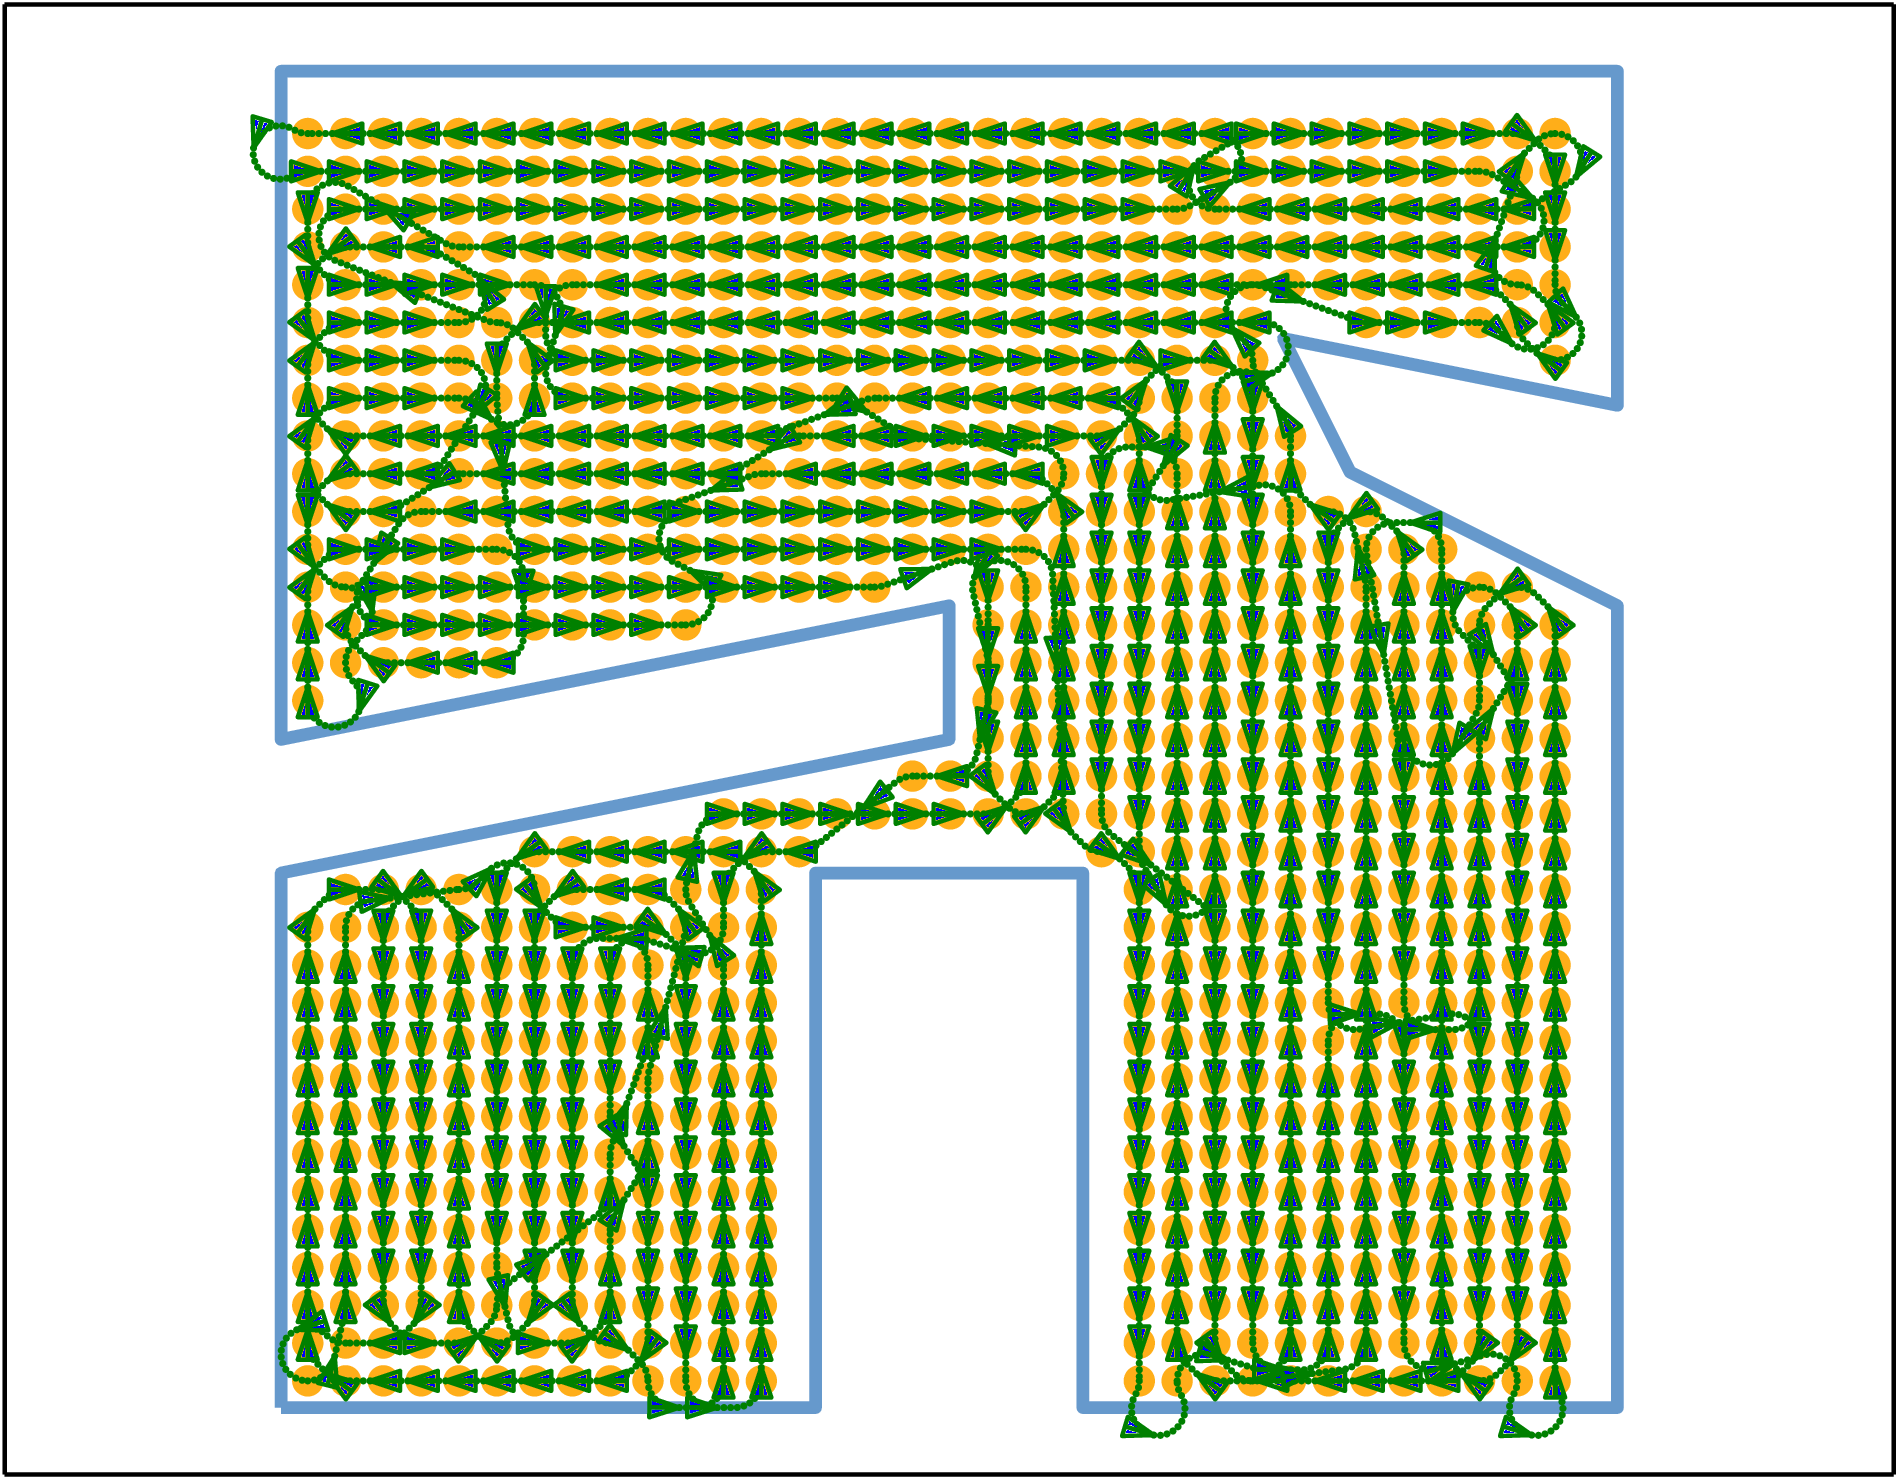
\includegraphics[width=0.3\textwidth]{img/chapter_4/point_10_coverage.png}% 
		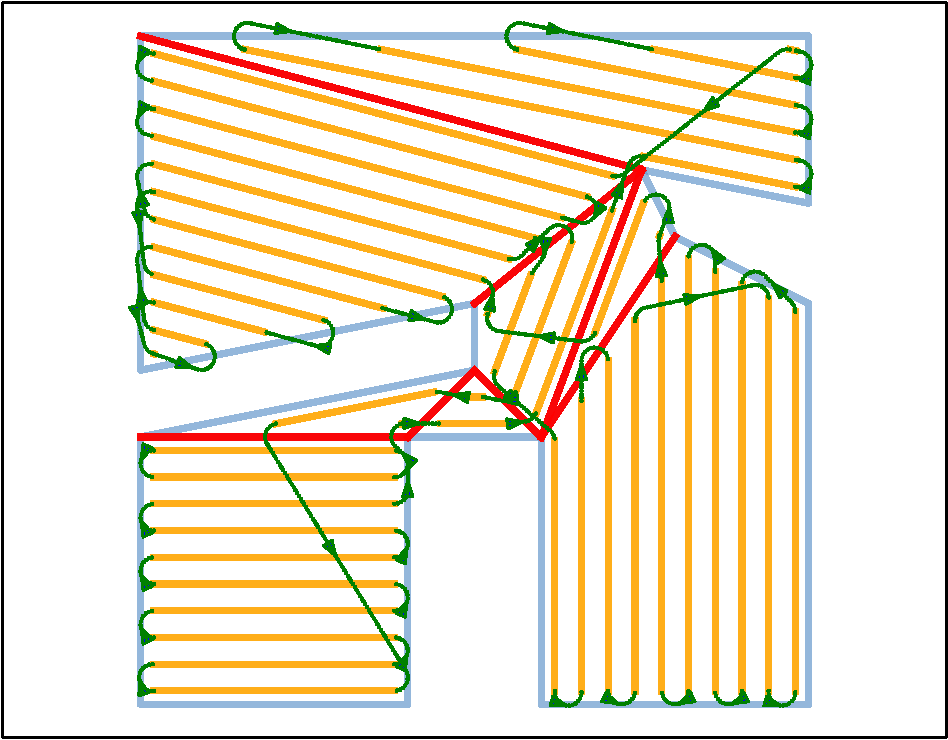
\includegraphics[width=0.3\textwidth]{img/chapter_4/greedy_10_coverage.pdf}% 
		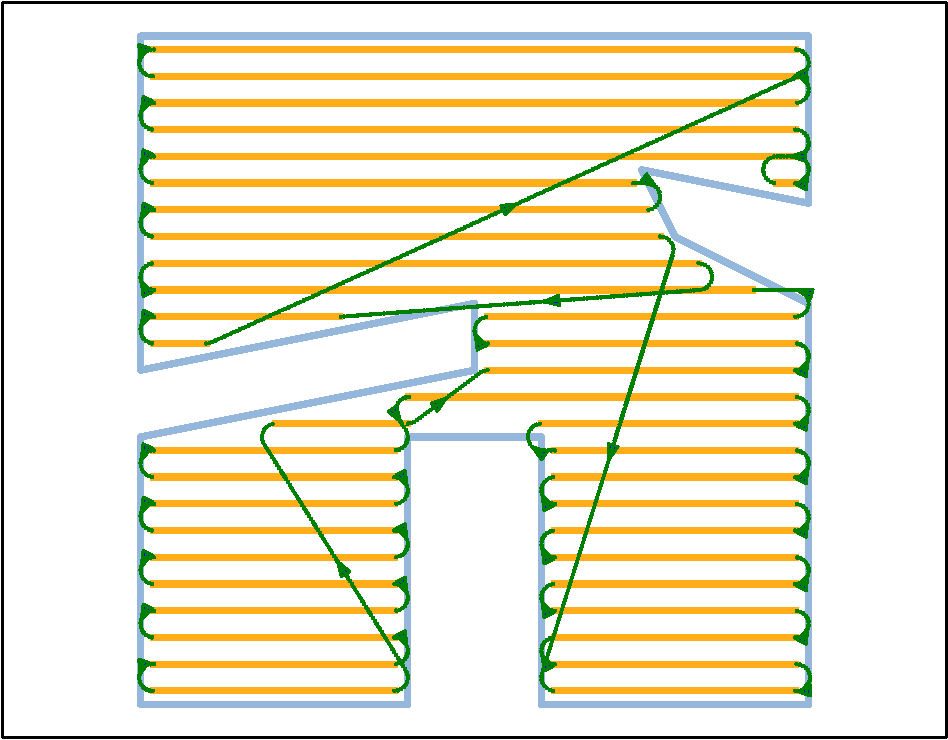
\includegraphics[width=0.3\textwidth]{img/chapter_4/min_10_coverage.pdf}

		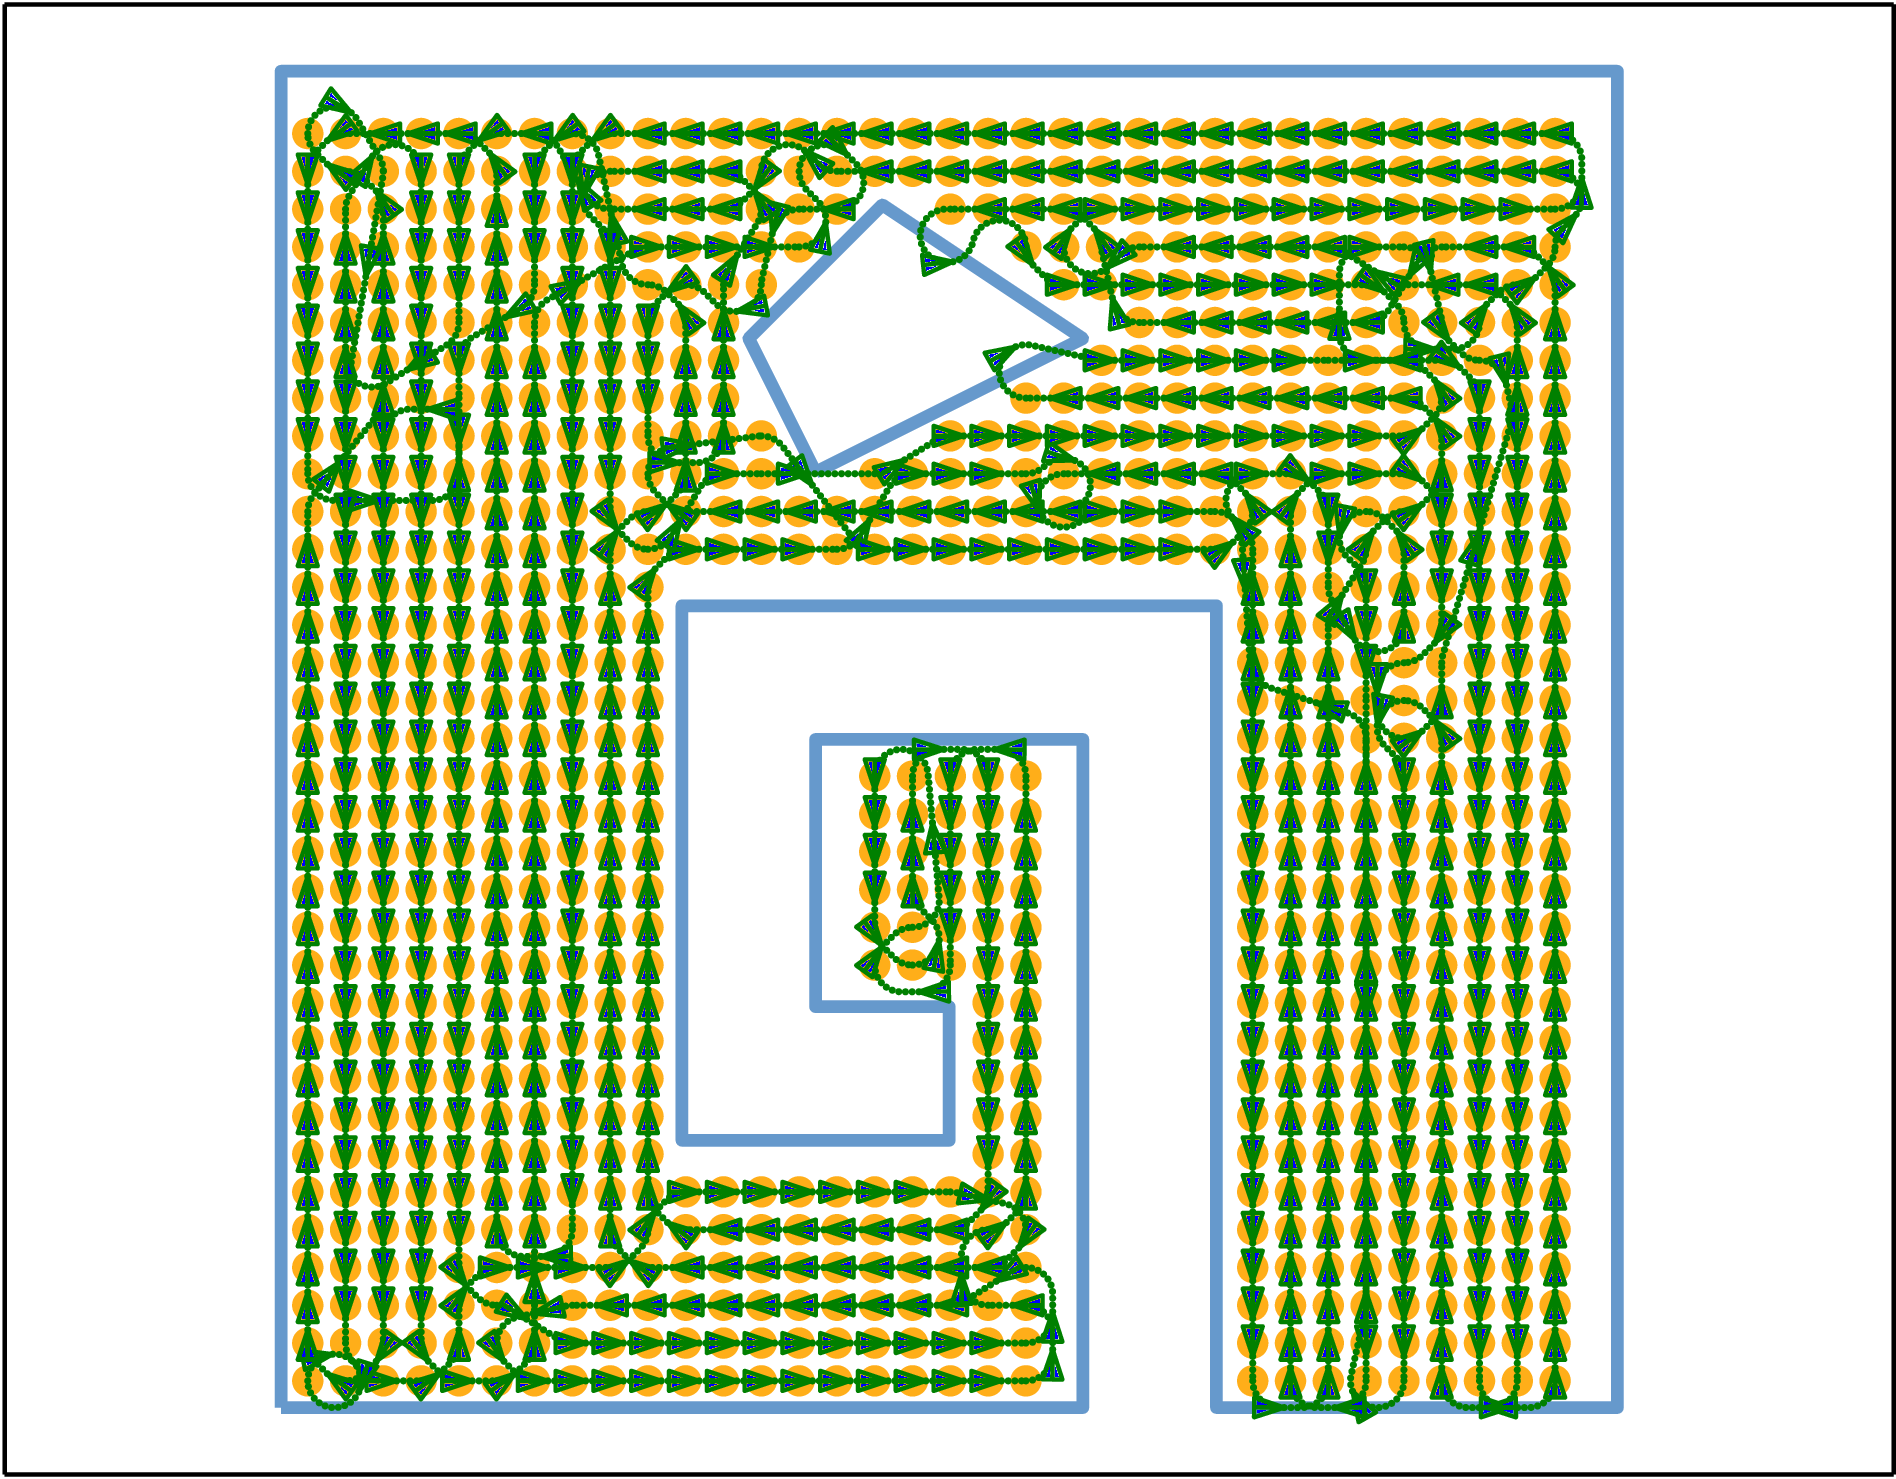
\includegraphics[width=0.3\textwidth]{img/chapter_4/point_11_coverage.png}% 	
		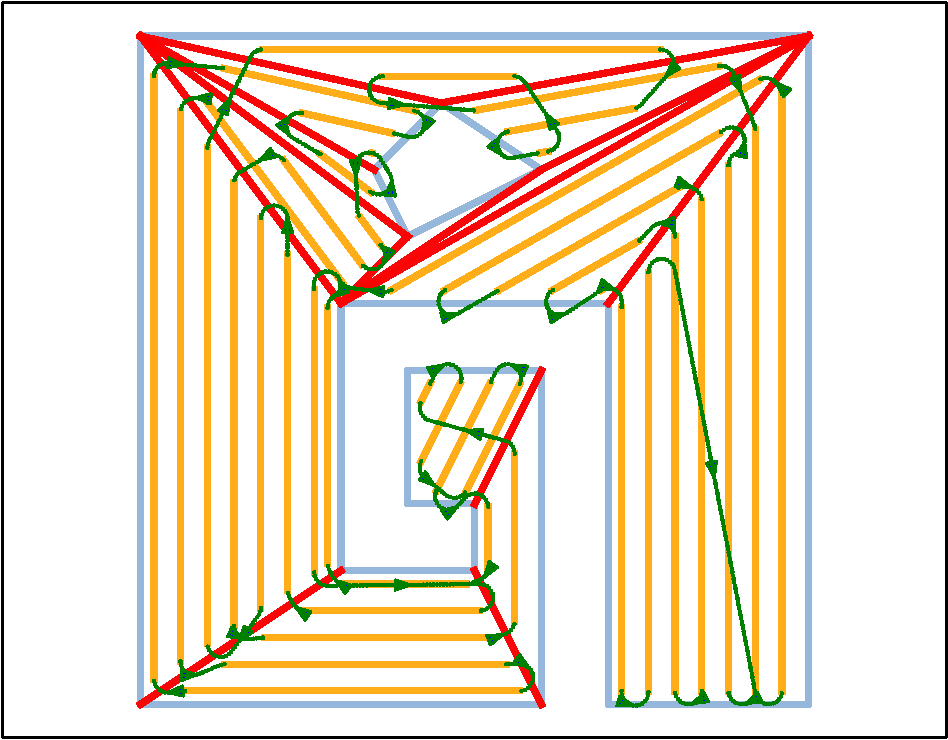
\includegraphics[width=0.3\textwidth]{img/chapter_4/greedy_11_coverage.pdf}%
		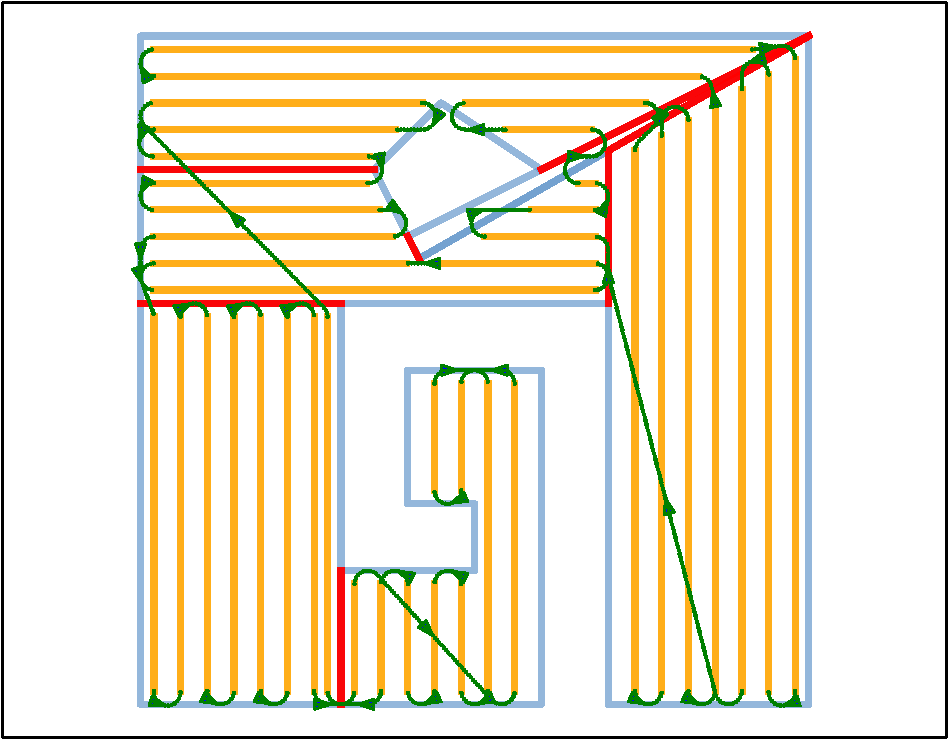
\includegraphics[width=0.3\textwidth]{img/chapter_4/min_11_coverage.pdf}

		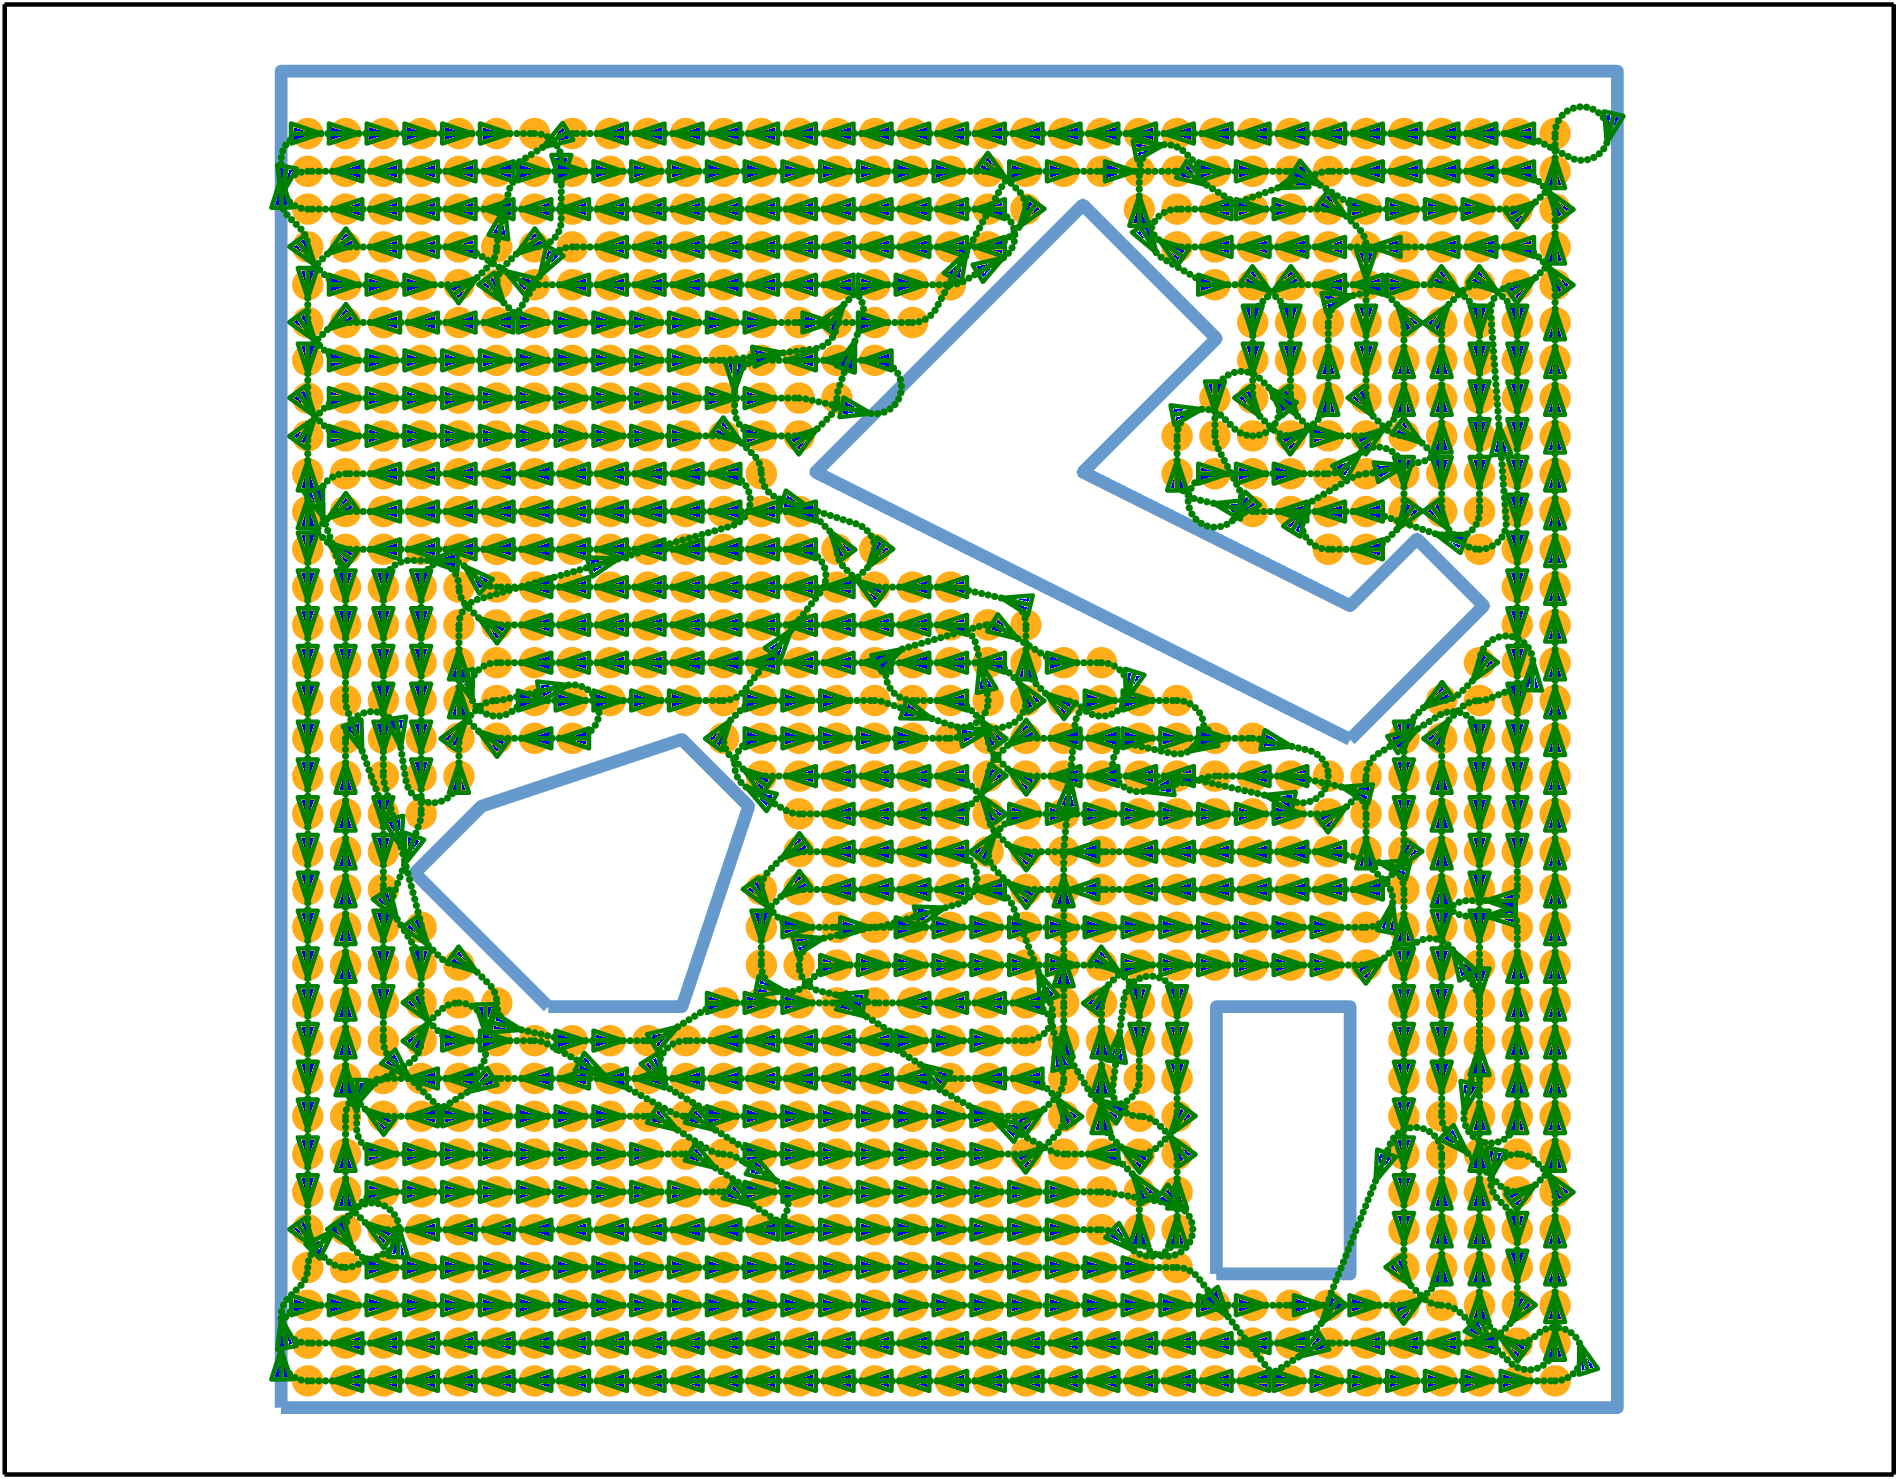
\includegraphics[width=0.3\textwidth]{img/chapter_4/point_12_coverage.png}%
		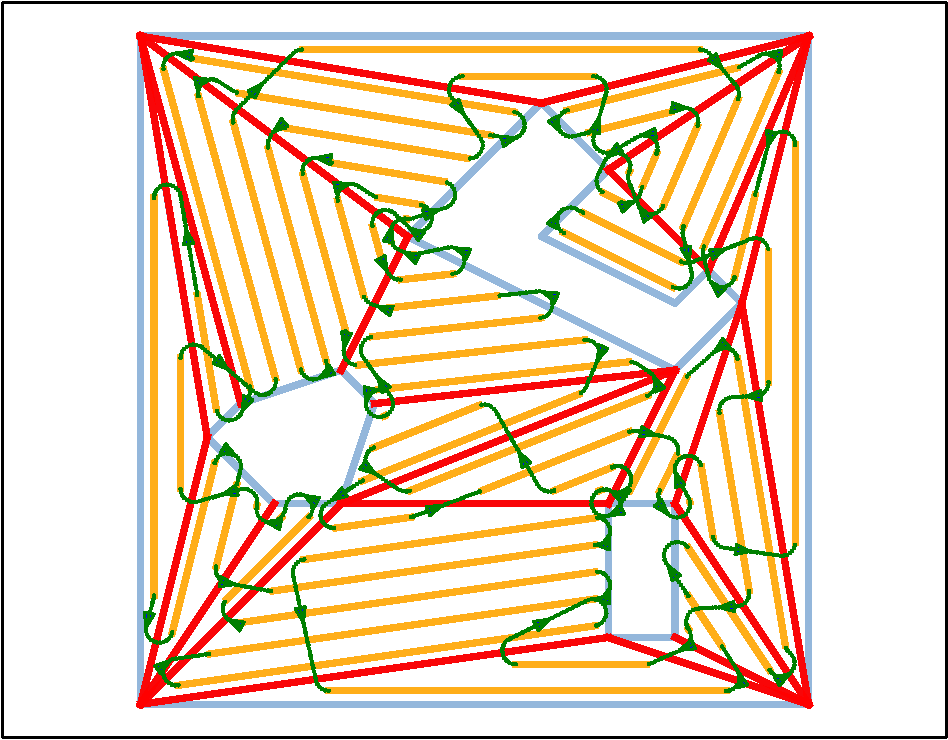
\includegraphics[width=0.3\textwidth]{img/chapter_4/greedy_12_coverage.pdf}%
		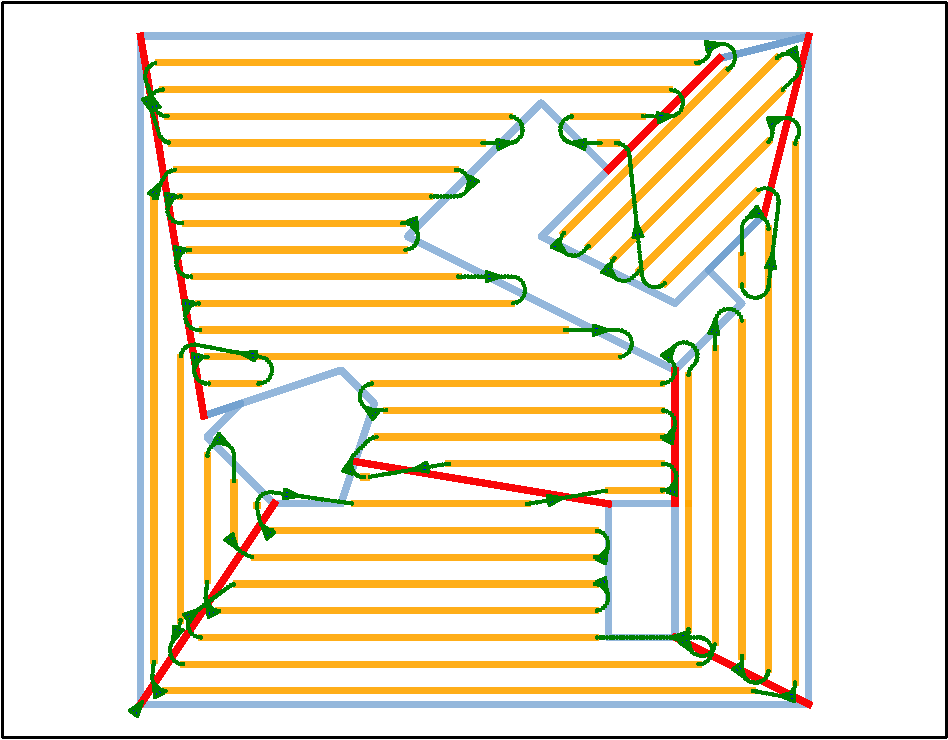
\includegraphics[width=0.3\textwidth]{img/chapter_4/min_12_coverage.pdf}

		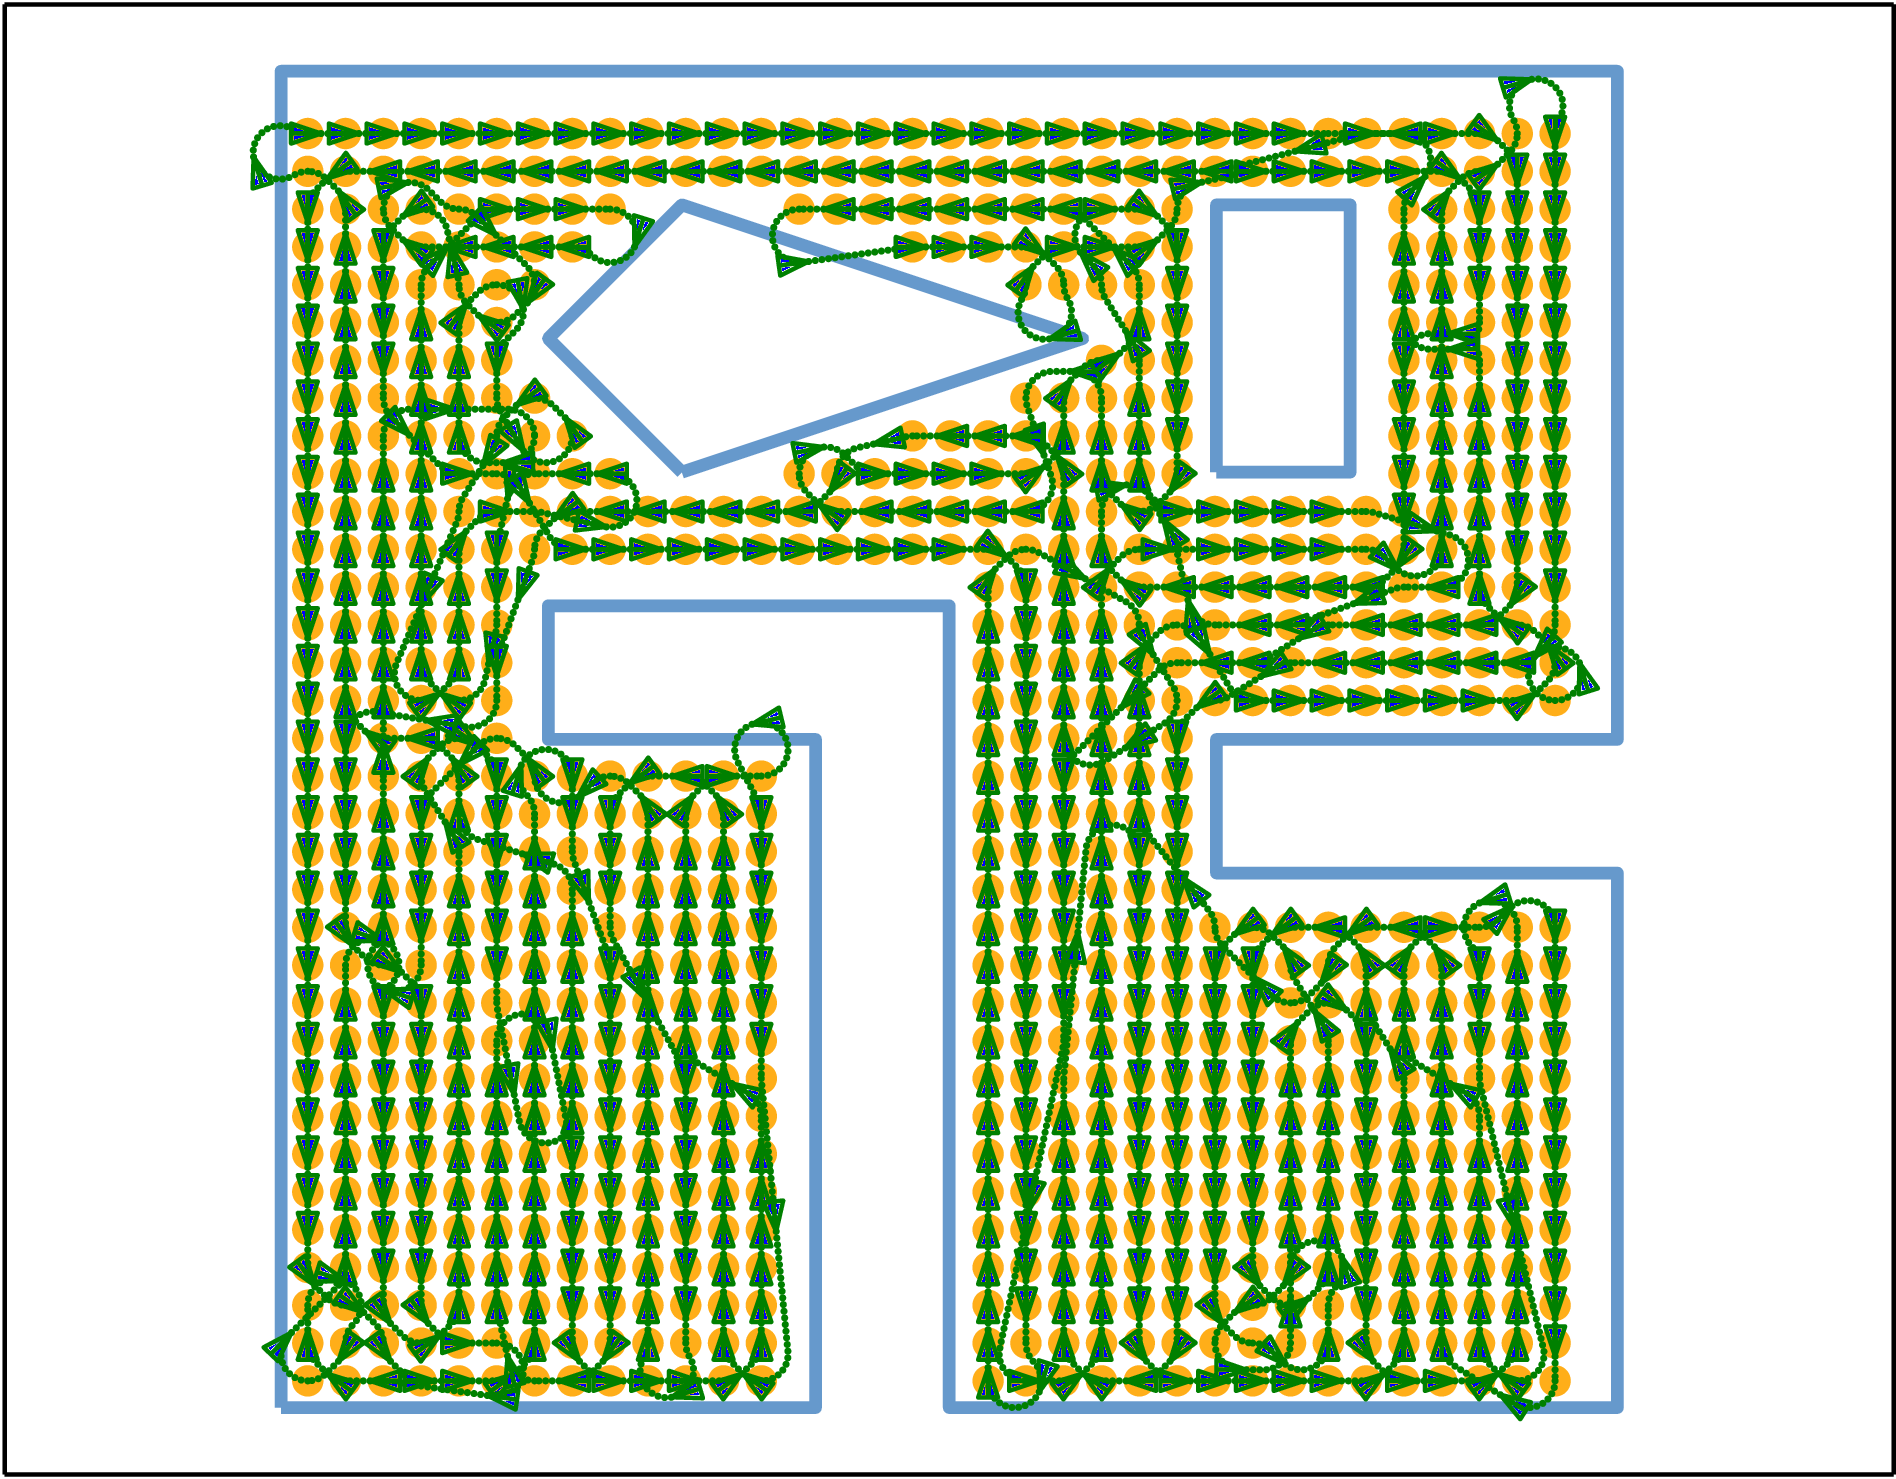
\includegraphics[width=0.3\textwidth]{img/chapter_4/point_13_coverage.png}%
		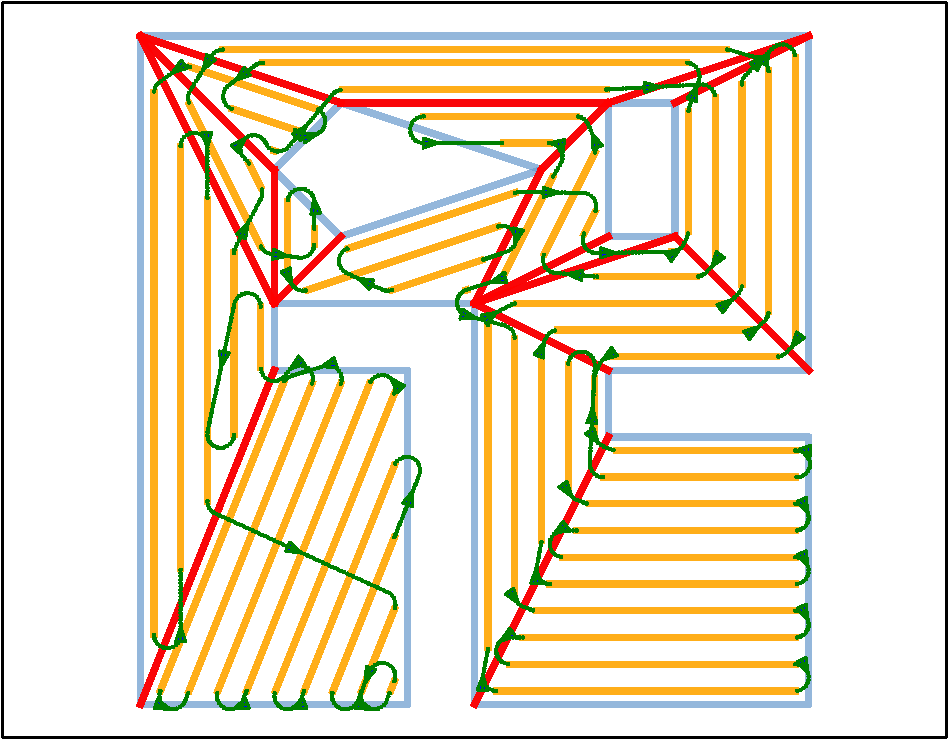
\includegraphics[width=0.3\textwidth]{img/chapter_4/greedy_13_coverage.pdf}% 
		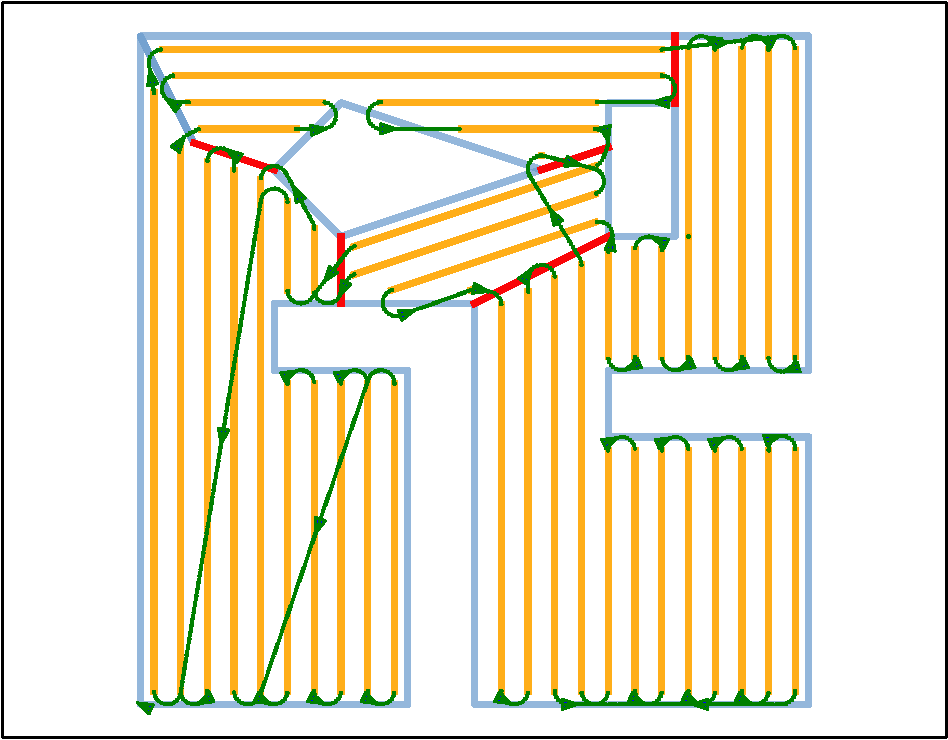
\includegraphics[width=0.3\textwidth]{img/chapter_4/min_13_coverage.pdf}
	\caption{First column: point decomposition. Second column: greedy decomposition. Third column: min altitude decomposition.}
	\label{fig:coverage_results}
\end{figure*}

\end{document}